\chapter{Hauptteil}
\label{c:hauptteil}

This chapter will first outline the problems that constitutes the main portion of this work. Each problem is described separately starting with the available data sources followed by a detailed description of the proposed solutions. After that, the proposed solutions are evaluated by empirical means and the results are presented. Performance studies are conducted to provide suitable recommendations concerning the real world application.



\section{Erlaeuterung der Aufgabenstellungen}
\label{s:erlaeuterungaufgabe}




\section{Aufgabe 1: Implementierung einer Browser-Extension zur Anzeige von Datenschutzinformationen im PlayStore}
\label{s:implementierungextension}

\subsection{Anwendungsszenario}
\label{ss:anwendungsszenario}

QUELLE STATISTIK? 

Während vor einigen Jahren Applikationen hauptsächlich auf eigenen Webseiten zum Download angeboten wurden, haben sich die
AppStores mitlerweile durchgesetzt. Vorteile für diese Plattformen sind unter anderem: erleichterter Zugang, Vergleiche mit anderen Applikationen und individuelle Empfehlungen. Bei der Wahl für eine bestimmte Applikation achten Nutzer auf Aspekte, wie Preis, Anzahl der Downloads und Bewertungen von anderen Nutzern.

Immer wichtiger aber auch die Frage: Welche Daten gebe ich der Applikation frei und wie werden diese verarbeitet. Der PlayStore bietet zwar einen groben Überblick, welche Daten eine Applikation von dem Handy ausließt, aber nicht wie diese vom Anbieter verarbeitet werden.

Dadurch entstehen beim Nutzer Fragen, welche der Playstore nicht beantwortet:
 \begin{enumerate}
 	\item Handhabung der Daten: Wie werden die Daten verarbeitet und an wen werden diese weitergeleitet? Wird ein Profil anhand der Daten erstellt? Welche Sicherheit besteht bei der Übertragung der Daten?
 	\item Vor- und Nachteile der Datenverarbeitung: Kann der Anbieter die Applikation dadurch komfortabler gestalten? Wird Werbung in der Applikation personalisiert? Besteht Gefahr vor Missbrauch der Daten?
 	\item Kontrolle über die Daten: Welche Möglichkeiten stehen zu Verfügung im Falle von Nichteinverständnis? Ist der Umgang mit den Daten nach der Installation noch einschränkbar. Kann der Nutzer die Verwendung der Daten verbieten und trotzdem die App weiterhin nutzen?
 \end{enumerate}


\subsection{Anforderungsanalyse}
\label{ss:anforderungsanalyse}

\subsubsection{Funktionale Anforderungen}

Aus den Fragen die bei dem Anwendungsszenario entstanden sind werden funktionale Anforderungen gebildet um konkrete Aufgaben für die Extension zu schaffen. -Anforderungen in TEXTFORM-

-Direkt bei Apps in Anforderungen erwähnen
\begin{itemize}
	\item[/F10/] Erweiterung der Informationen im PlayStore:
	Der Nutzer hat die Möglichkeit im Browserfenster per Aktivierung bzw. Deaktivierung der Extension zusätzliche Datenschutzinformationen zu den angezeigten Applikationen ein- bzw. auszublenden.
	\item[/F20/] Anzahl von bedenklichen Eigenschaften einer Applikation:
	Zu jeder Applikation erhält der Nutzer ein Feedback von der Extension, wieviele Bedenken vorliegen.
	\item[/F30/] Darstellung von kritischen Eigenschaften einer Applikation:
	Eigenschaften einer Applikation, welche einen erheblichen Nachteil für den Nutzer darstellen oder einen möglichen Gesetzesverstoß beinhalten werden hervorgehoben.
	\item[/F40/] Abrufen von Details zu den Bedenken:
	Wird ein Bedenken angezeigt, kann der Nutzer direkt Erläuterung, Handlungsempfehlung sowie Vor- und Nachteile zu diesem Bedenken abrufen.
	\item[/F50/] Empfehlung bei Suchanfragen:
	Basierend auf den Bedenken einer Applikation kann der Nutzer die Suchanfrage so anpassen, dass ihm unbedenkliche Applikationen priorisiert angezeigt werden.
\end{itemize}

\subsubsection{Nichtfunktionale Anforderungen}
Das Programm richtet sich in erster Linie an Nutzer, denen keine besonderen informatischen Kenntnisse abverlangt werden
Extensions zeichnen sich durch ihre Einfachheit aus. Nutzer wissen vor der Installation, welche Funktionen diese Programme haben. Die Extension soll auf den ersten Blick klar machen, welche Komponenten des Browsers erweitert oder verändert wurden.
-QUELLE- Was ist eine Nichtfunktionale Anforderung + kurze Auflistung (BUCH)
\begin{itemize}
	\item[/NF10/] Darstellung und Einbindung der Informationen
	Darstellung und Einbindung spielen bei Browser-Extensions eine wichtige Rolle. Hier wird keine grundlegend neue Oberfläche gestaltet sondern eine bereits vorhandene erweitert. Der Fokus fällt darauf, die bestehende Oberfläche so zu verändern, dass alle Elemente der Extension an der richtigen Stelle eingebaut werden. Der Nutzer soll auf den ersten Blick erkennen welche neuen Informationen zu welchen bereits bestehenden Teilen der Website gehören.
	\item[/NF20/] Persistenz der Website
	Im Gegenspiel zu NF10 darf die Website nicht so verändert werden, dass sie in ihrem Aussehen und ihren Funktionen zu stark von ihrem Originalzustand abweicht. Gerade bei Seiten auf denen viele Elemente automatisch generiert werden, verursachen kleine optische Veränderungen schon Probleme beim Aufbau der Website. Entsprechend müssen Informationen so subtil wie möglich eingebettet werden. So wird verhindert, dass der Nutzer die Extension nur aufgrund der Optik wieder deinstalliert.
	\item[/NF30/] Handhabung
	In der Extension werden viele und vor allem auch umfangreiche Informationen angeboten. Diese dürfen den Nutzer nicht überwältigen. Dennoch müssen sämtliche Punkte vgl pguard informationen an der richtigen Stelle zur Verfügung stehen.
	\item[/NF40/] Skalierbarkeit
	def Skalierbarkeit? Hier bezieht sich der Begriff Skalierbarkeit vor allem auf Anfragen an das Backend. Angenommen die Extension erreicht eine hohe Nutzerzahl. Dadurch steigt das Risiko auf Überlastung des Servers. Um das zu verhindern werden bei der Informationsgewinnung zwei Aspekte besonders wichtig. Zum Ersten wie aktuell die Informationen sein sollen. Je aktueller, desto öfter müssen Anfragen gesendet werden. Zum Anderen die Relevanz. Wie schnell müssen welche Informationen vorhanden sein und welche Informationen, die eine Analyse erfordern, werden erst auf spezielle Anfrage des Nutzers angefragt. Diese Anforderung stellt einen zentralen Punkt in der Entwicklung der Extension dar und wird in Aufgabe 2 detailliert behandelt.
	\item[/NF50/] Datenschutz
	Bei allen Webdiensten spielt der Datenschutz eine wichtige Rolle. Auch in diesem Programm sollen Daten gespeichert werden um die Anforderung /NF40/ zu unterstützen. Um Datenschutzbedenken auszuschließen muss das Format der Daten so gewählt werden, dass diese nicht personalisert werden und nach Möglichkeit komplett lokal gespeichert werden.
	\item[/NF60/] Korrektheit der Daten
	Alle Informationen zu Applikationen die dieses Programm darstellt werden extern von einem Server des privacy guard-Projekts eingespeist. Dieser gewinnt die Daten hauptsächlich auf automatischen Textmining-Verfahren. Ein Problem bei diesen Verfahren ist die fehlenden Validierung der Informationen. Ursachen wie das heterogene Format von Datenschutzerklärungen und Mehrfachverlinkungen von Datenschutzinformationen können zu bei dieser Methode zu Fehlern oder Ungenauigkeiten führen. Aus diesem Grund muss dem Nutzer verdeutlicht werden, dass alle Angaben als Empfehlungen zu betrachten sind und keine verbindlichen Aussagen über Applikationen getätigt werden.
\end{itemize}

\subsection{Programmaufbau}
\label{ss:programmaufbau}
Die Struktur des Programms orientiert sich an der beschriebenen Architektur in Kapitel~\ref{ss:darstellung}. Dieser Abschnitt befasst sich mit der Umsetzung der Anforderungen, welche im vorangegangen Kapitel aufgesetzt wurden. Dabei werden wichtige Eigenschaften aus an Teilen des Quellcodes betrachtet und getroffene Entscheidungen begründet. Außerdem werden kritische Stellen beleuchtet, welche für die Diskussion und fortführende Arbeit relevant sind.


\lstinputlisting[label={src:manifest}, caption={Aufbau der manifest.json}]{../../Extension/src/manifest.json}

Das Manifest stellt die grundlegenden Zusammenhänge der Extension dar. Unter anderem den gewählten Entwicklungsnamen der Extension "PGuard AppRating" und die entsprechende Beschreibung.
Weiterhin sind die nötigen Berechtigungen aufgeführt.
\begin{itemize}
	\item storage:
	Berechtigung zum Zugriff auf Speicherplatz, um Informationen aus Backend-Anfragen zu speichern. Details dazu in Kapitel~\ref{ss:anforderungen}.
	\item declarativeContent:
	Bereitstellung von Events, wie Seitenaufruf oder -änderung und damit zusammenhängende Regeln, wie das Ausführen von Content-Skripten. Diese API wird vom Background-Skript genutzt,welches die genannten Aufgaben umsetzt.
	\item activeTab und tab:
	Gibt an, ob sich der Nutzer gerade in einem Tab befinden auf dem die Extension aktiv ist.
\end{itemize}
Außerdem werden alle Dateien ihren Rollen zugewiesen.
\begin{itemize}
	\item Content-Skript:
	Unter dem Punkte "content scripts" wird festgelegt, welche Skripte unter welchem URL aktiv sind. Der Ausdruck 
	"*://play.google.com/store/apps*" 
	bedeutet, dass die Extension auf jeder Playstore-Seite der Kategorie Apps und deren Unterverzeichnis aktiv ist. Da es sich um eine page action Extension handelt, wird lediglich eine Website als "match" aufgeführt. Die beiden wichtigen Dateien hier sind "pguard.js" als das Content Skript für sämtliche Funktionen die die Erweiterung der Website betreffen und "popup-controller.js" für alle Funktionen des Popups. Hinzu kommen sämtliche Bibliotheken, welche von den Content-Skripten benötigt werden.
	\item Background-Skript
	Wie bereits erwähnt fungiert das Background-Skript "background.js" als Eventhandler der Extension ist deshalb separat im Manifest aufgeführt.
	\item web\_accessible\_resources
	Diese Ressourcen sind Dateien welche der Extension zur Verfügung stehen aber selber keine Skripte sind. Sie beinhalten ausgelagerte Informationen wie Fließtexte und Templates zum Bauen von HTML-Elementen. Die "popup.html" ist hier ein Sonderfall und wird direkt dem Popup zugewiesen.
\end{itemize}

Die Background.js besteht lediglich aus Callback-Funktionen der declarativeContent API. Hier wird zur Installation der Extension ein Listener eingebunden. Dieser funktioniert mit Regeln nach dem Konditionen-Aktionen-Prinzip. Zum Start des Aufrufs werden alle bereits vorhandenen Regeln des Listeners entfernt und anschließend die übergebenen Regeln installiert.
Hier benötigt das Programm eine Regel. Die Kondition prüft ob der passende URL aufgerufen wurde. Dieser stimmt mit dem String aus der Manifest-Datei überein. Ist die Kondition erfüllt, aktiviert sich das Popup.


\lstinputlisting[label={src:background}, caption={background.js}]{../../Extension/src/background.js}




\subsection{Ergebnis}
\label{ss:ergebnisseht1}

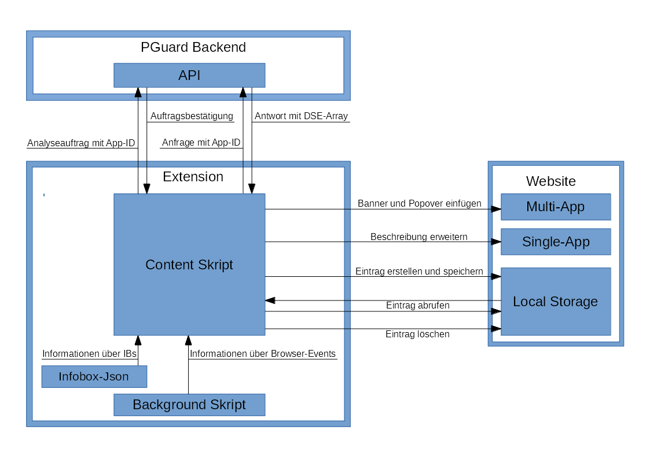
\includegraphics{pics/Aufbau.png}

\subsection{Diskussion}
\label{ss:diskussionht1}










